\documentclass{article}
\usepackage[utf8]{inputenc}
\usepackage[catalan]{babel}
\usepackage{hyperref}
\usepackage{graphicx}
\usepackage{subfiles}
\usepackage{comment}
\usepackage{titlesec}
% caption and subcaption work together
\usepackage{subcaption} % loads the caption package
\setcounter{secnumdepth}{4}

% Code
\usepackage{listings}
\usepackage{minted}
\usepackage{xcolor}

% Ploting 
\usepackage{pgfplots}
\usepackage{pgfplotstable}
\usepackage{booktabs}
\usepackage{array}
\usepackage{colortbl}

% Ploting settings
\pgfplotstableset{ 
  % global config, for example in the preamble
  every head row/.style={before row=\toprule,after row=\midrule},
  every last row/.style={after row=\bottomrule},
  fixed,precision=2,
}

% Code settings
\definecolor{codegreen}{rgb}{0,0.6,0}
\definecolor{codegray}{rgb}{0.5,0.5,0.5}
\definecolor{codedarkgray}{rgb}{0.75,0.75,0.75}
\definecolor{codepurple}{rgb}{1,0,0}
\definecolor{codedarkpurple}{rgb}{0.65,0,0.8}
\definecolor{codedarkorange}{rgb}{0.85,0.4,0}
\definecolor{backcolour}{rgb}{0.95,0.95,0.95}

\lstdefinestyle{mystyle}{
    frame=tb,
    language=[Sharp]C,
    backgroundcolor=\color{backcolour},   
    commentstyle=\color{codegray},
    keywordstyle=\color{codedarkorange},
    numberstyle=\tiny\color{codegray},
    stringstyle=\color{codegreen},
    basicstyle=\fontsize{9}{10}\selectfont\ttfamily,
    breakatwhitespace=false,         
    breaklines=true,                 
    captionpos=b,                    
    keepspaces=true,                 
    numbers=left,                    
    numbersep=5pt,                  
    showspaces=false,                
    showstringspaces=false,
    showtabs=false,                  
    tabsize=2,
    literate={\ \ }{{\ }}1
}
\lstset{style=mystyle}

\setlength{\parskip}{0.5em}

\titleformat{\paragraph}
{\normalfont\normalsize\bfseries}{\theparagraph}{1em}{}
\titlespacing*{\paragraph}
{0pt}{3.25ex plus 1ex minus .2ex}{1.5ex plus .2ex}

%%------- Definició de l'estructura del titol -------%%
\title{ \textbf{ Aprenentatge per reforç amb Unity} 
\\ {\Large TAIA Project}}
\author{\small Wilber Eduardo Bermeo Quito }
%\date{\small Entrega: 5 de decembre 2021}


% Canvi de nom a la taula de continguts
\renewcommand*\contentsname{Taula de continguts}
\renewcommand\vdots{\vbox{\baselineskip3pt\lineskiplimit0pt\kern1pt\hbox{.}\hbox{.}\hbox{.}\kern-1pt}}

%%------- Inici del documents -------%%
\begin{document}

\maketitle

 % Titol
    \maketitle
    \thispagestyle{empty}
    \newpage
    
    % Taula de continguts
    \tableofcontents
    \newpage
    
    %% ---- start documentation ---- %%
    
    \section{Problema a resoldre en una frase}
    
    Fer que un NPC segueixi una política en concret fent ús de Deep Reinforcement Learning en Unity.

    \section{Introducció i Motivació}
    
    Durant l’estiu del 2021 m’he estat barallant amb Unity (motor de videojocs) perquè vull fer un joc com a treball final de grau.
    
    El joc, resumidament, serà un Metroidvania 2D, en el qual hi haurà una tira de diferents NPCs. Molts d’aquests NPCs seran personatges actius i enemics.

    La motivació és clara, aprendre més d'Unity i expandir la riquesa del TFG amb les eines pròpies d’Unity que dona per implementar intel·ligència artificial als videojocs.  
    
    \section{Dades/Coneixements dels que es disposa}
    
    Degut a la naturalesa del problema seleccionat, no es necessiten conjunts de dades per poder treballar.

    Conec l'entorn de treball Unity, no professionalment, però si tinc un base.
    
    El que em permetrà encarar el problema és l'eina \textit{ML-Agents Toolkit}. Dona totes les eines necessàries per utilitzar Unity com a motor de simulació perquè els Agents de les escenes aprenguin polítiques segons una modelització del problema a resoldre.
    
    \newpage
    
    \section{Proposta}
    
    \subsection{Agent}
    Classe que conté mètodes que poden ser sobre escrits. La seva API contempla mètodes per poder generar observacions del medi, per prendre accions i per assignar recompenses.

    La classe Agent conte altres mètodes que poden ser sobre escrits. Cada Agent està relacionat amb un Behavior Parameter class i a un Decision Requester.
    
    \subsubsection{Com modelitzar un Agent?}
    Es necessiten definir tres tipus d’entitats per cada moment en el joc.
    
    \begin{itemize}
        \item Observacions
        \item Accions
        \item Recompenses
    \end{itemize}
    
    \paragraph{Observacions}
    
    Les observacions poden ser numèriques o visuals. Les observacions numèriques són del punt de vista de l'observador (NPC), les visuals en canvi, són generades per col·lisions de rajos que es poden ajuntada a l'agent i representen el que l'agent està veient en aquell mateix moment.
    
    \paragraph{Accions}
    
    El que realment l'agent pot fer dintre de l'escena. Les accions poden ser representades per valors continus o discrets.
    
    \paragraph{Recompenses}
   És un escalar que representa que tan bé ho està fent l'agent. Les recompenses (negatives o positives) no tenen per què ser donades a cada moment, es poden donar en certs moments provocats per esdeveniments. És important saber quan i quant es recompensa o es castiga a l'agent pel seu acte. Depenent de la política de recompenses farà que l'aprenentatge d'una certa tasca sigui més ràpida o més lenta.
    
    \subsection{Polítiques a aprendre}
   Els següents dos punts són els problemes a modelitzar perquè l'Agent aprengui la política adequada per compliar-los.
    
    \subsubsection{Autonomia en el moviment}
    
    L'NPC ha de ser capaç de moure d'esquerra a dreta de manera cíclica. El radi de desplaçament respecte al punt origen ha de ser configurable.

    Arribar al màxim rang de desplaçament tant d'esquerra a la dreta ha de donar feedback positiu, però no ha de passar que es quedi en un extrem sense moure, només s'ha de poder atorgar feedback positius i s'ha vingut de l'altre extrem, un cas excepcional seria la primera vegada que apareix en l'entorn del joc, ja que surt del centre del desplaçament.
    
    En cas de col·lisions amb objectes que no siguin targets d'atac dintre del seu rang ha de poder ser capaç de girar i fer el recorregut contrari.
    
    \subsubsection{Saber atacar}
    
    Un cop l'Agent hagi apres a moure's, la meva idea es que l’NPC detecti entitats a atacar.
    
    Aquestes entitats únicament seran detectables si estan dintre d'un rang esfèric que tindrà com radi el rang de desplaçament del NPC. L'objectiu en aquest cas es que, deixi de fer el moviment cíclic d'esquerra detrac i que salti sobre l'objectiu fent col·lisió, les col·lisions encertades donaran feedback positiu.
    
    \newpage
    
    \subsection{Arquitectura, Algorismes, Propostes existents}
    
    L'arquitectura del problema que abordo bé donat per les eines que utilitzo per resoldre-ho, en aquest cas \textit{ML-Agents Toolkit}. A part de les eines de \textit{ML-Agents Toolkit} faré servir \textit{Tensorboard} per veure les estadístiques d'aprenentatge.

    A continuació explicaré com és l'arquitectura de ML-Agents Toolkit. ML-Agents Toolkit té els següents quatre blocs com a estructura principal.
    
    \begin{itemize}
        \item Espai d'aprenentatge (Escena d'Unity)
        \item Comuniador (Broquer que connecta Unity amb l'API de Python)
        \item Python API
        \item Python Trainers
    \end{itemize}

    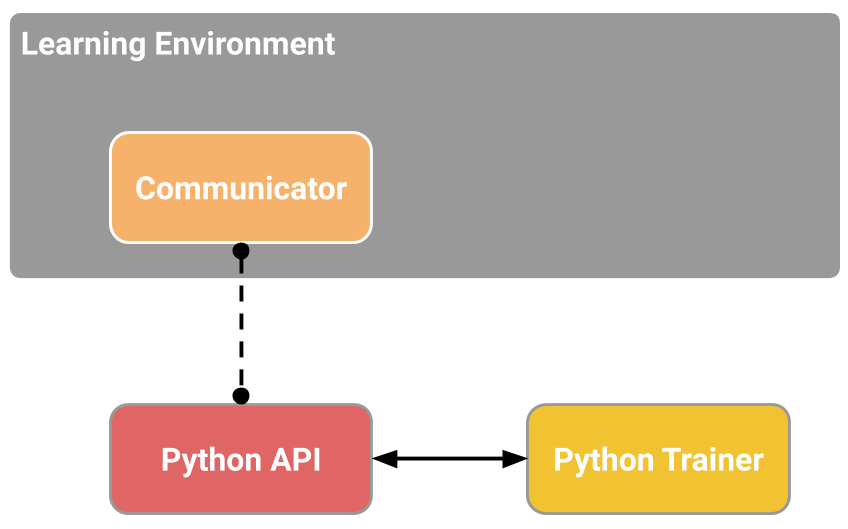
\includegraphics[width=\textwidth]{images/learning_environment_basic.png}
    
    \newpage
    
    \subsubsection{Espai d'aprenentatge}
    Aquí està l'escena d'Unity i els personatges. Els personatges que per requeriment del problema s'han definit com a Agents, podran observar, prendre decisions i tenir recompenses.
    
    \subsubsection{Agent}
    Aquí està l'escena d'Unity i els personatges. Els personatges que per requeriment del problema s'han definit com a Agents, podran observar, prendre decisions i tenir recompenses.
    \begin{itemize}
        \item Initialize
        \item OnEpisodiBegin
        \item OnActionReceived
        \item CollectObservations
        \item Heuristic
    \end{itemize}
    
    \newpage
    
    \paragraph{Initialize}
    Aquest mètode es crida un cop únicament en el cicle de vida de l'aprenentatge. Està pensat per fer caching d'objectes de l'escena o inicialitzar valors.
    
    \paragraph{OnEpisodiBegin}
    Aquest mètode es crida cada cop que un episodi d'aprenentatge ha acabat, forçadament o perquè el màxim nombre de passos de l'episodi s'han completat.
    
    \paragraph{OnActionReceived}
    Aquest mètode porta un paràmetre d'entrada, anomenat ActionBuffer, l'ActionBuffer, és un objecte que té dos arrays, un per poder representar valors continus i altres per representar valors discrets.
    
    Aquest mètode interactua tant amb el mètode \textit{heuristic} i amb el motor d'aprenentatge automàtic.
    
    \paragraph{CollectObservations}
    Aquest mètode s'executa cada x temps, aquest temps d'execució es configura amb l'eina d'Unity.
    
    El mètode té com a paràmetre una estructura de dades semblants com a paràmetre d'entrada que el mètode OnActionReceived. En aquest cas no està pensat per consumir les dades sinó per modificar aquesta referència i per donar informació al motor de Reinforcement Learning quan estem en mode de \textit{Learning}.


    \paragraph{Heuristic}
    Aquest mètode permet interactuar amb el jugador. Fixat que té la mateixa estructura de dades com a paràmetre que el mètode ActionBuffers.
    
    Els valors que s'emplenin en els buffers d'aquesta estructura de dades aniran a parar al mètode \textit{OnActionReceived}.
        
    \subsubsection{Behaviour}
    Script que esta pensat per parametritzar i relacionar l’Agent amb la configuració externa a Unity.
    
    Un Behavior pot tenir els següents comportaments:
    \begin{itemize}
        \item Learning
        \item Heuristic
        \item Inference
    \end{itemize}
    
  \paragraph{Learning}
    Quan el \textit{Behavior} està en mode \textit{Learning} vol dir que utilitza el model generat per la sobreescriptura dels mètodes de la clase \textit{Agent} per aprendre. En aquest mode Unity es connecta amb el procés de \textit{mlagents-learn} per generar la xarxa neuronal que representa l'aprenentatge del model.
    
    \paragraph{Heuristic}
    En aquest mode no hi ha procés d'aprenentatge, es fa servir la funció \textit{heuristic} de la classe \textit{Agent} per interactuar amb l'Agent.
    
    \newpage
    
   \paragraph{Inference}
    Quan el \textit{Behavior} està en mode \textit{Inference} implica que hi ha una xarxa neuronal amb una política apresa, i l'objecte que té aquesta xarxa neuronal es comportarà segons el que s'hi hagi après.
    
    \subsubsection{Requester}
    És un Script que serveix per forçar que l'Agent prengui decisions, sense aquest Script com a Component en el nostre Agent, l'Agent mai prendrà decisions. Aquí es pot configurar el període de decisions.
    
    En la següent imatge hi ha les tres diferents arquitectures que podem tenir segons quin comportament tingui el component \textit{Behavior} del objecte Agent. \\
    
    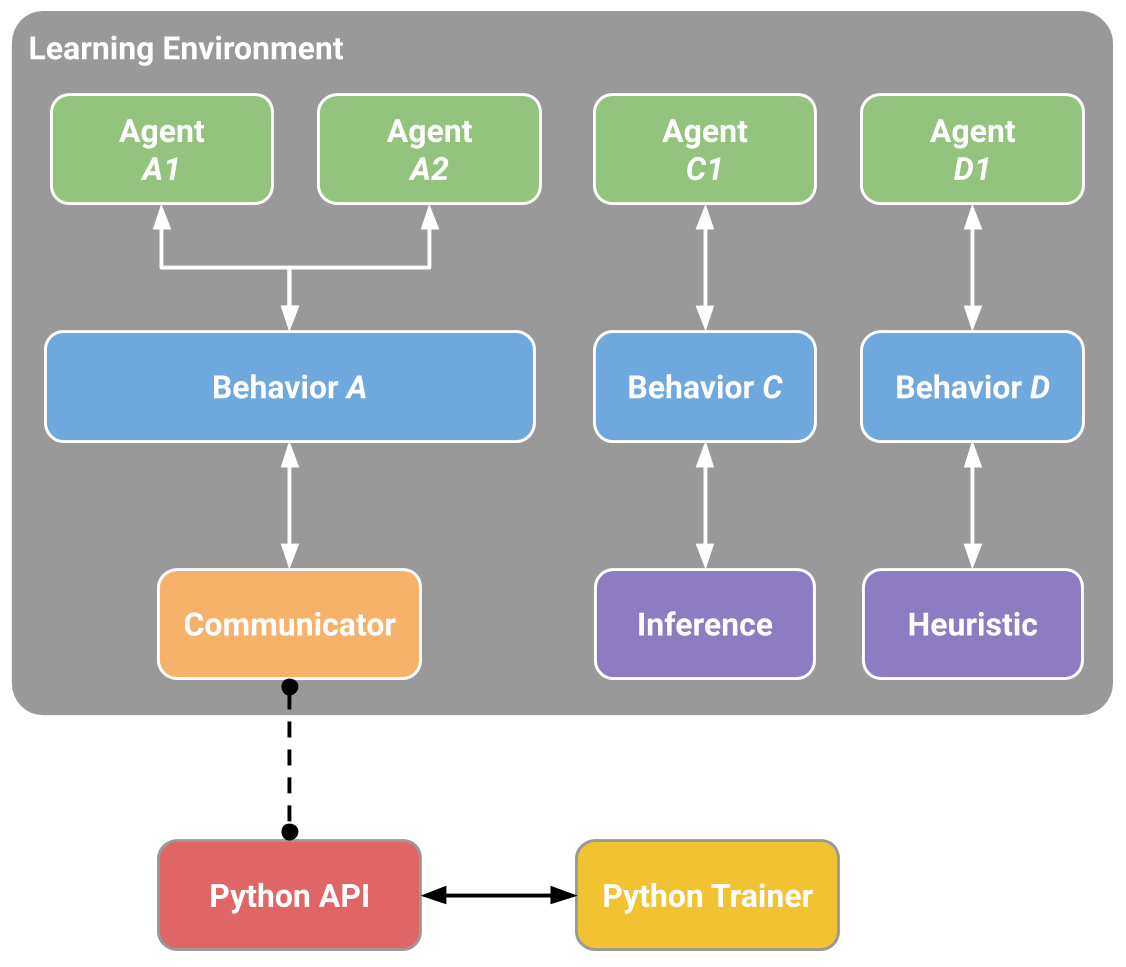
\includegraphics[width=\textwidth]{images/arquitecture_mlagent.png}
    
    \newpage
    
    \subsubsection{Tensorboard}
    Quan l'entrenament s'està executant, ML-Agents Toolkit guarda estadístiques dintre del directori resolts en un directori amb nom únic, donat a l'hora d'executar el procés mlagents-learn.

    Per observar el procés d'entrenament quan està corrent el procés o quan no, ens apropem a la carpeta de resultats i executem: tensorboard –logdir */results\$\{training id\}.
    
    Això obrirà un servidor per servir el contingut estàtic en un dels ports de la teva màquina.
    
    Explicaré alguna de les gràfiques que \textit{Tensorboard} genera, ja que molt segurament les veurem més endavant en cada un de les versions de l'Agent.
    
    \paragraph{Cumulative Reward}
    Gràfica que representa la mitja de el que guanya l'Agent per episodi. Un bon procés d'aprenentatge gènera una gràfica ascendent que en algun moment s'estanca, ja que la seva mitja per episodi és manté.
    
    \paragraph{Episodi Length}
    Representa la durada mitjana per episodi. Aquesta gràfica depèn de la implementació del model, ja que segons la característica del problema es pot forçar el reinici d'episodi, o potser el problema és maximitzar o minimitzar el temps de vida de l'Agent.
    
    \paragraph{Policy Loss}
    Representa quan la política de l'Agent canvia, un model correcte tendirà a fer una gràfica descendent.
    
    \paragraph{Entropy}
    Representa que tan aleatoris són els moviments de l'Agent, un model correcte expressa una gràfica d'Entropia descendent, ja que significa que realment està aprenent una política i no està fent tants d'intents per provar coses noves.
    
    \newpage
    
    \textbf{Arquitectura final}
    
    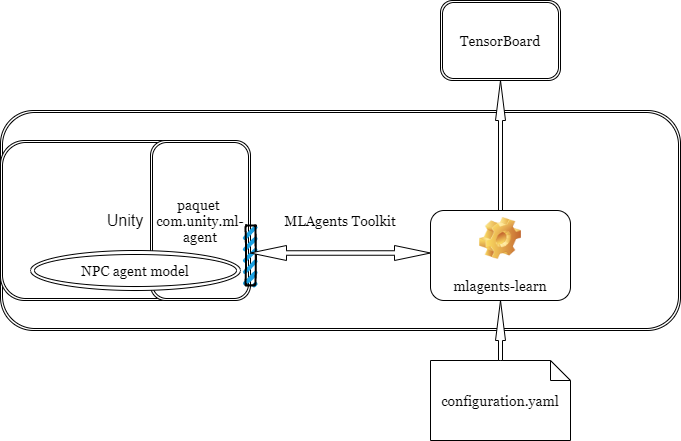
\includegraphics[width=\textwidth]{images/arquitectura-tools.drawio.png} 
    
    \newpage
    
    \section{Experiments}
    
    Aquest projecte conté un seguit d'experiments basats en fases.
    Les fases venen donades per l'apartat \textit{4.2 Polítiques a aprendre}.
    
    \subsection{ Representació de l'objecte NPC dintre d'Unity }
    L'objecte NPC està format tres objectes fills.
    
    \begin{itemize}
        \item Limit esquerra
        \item Limit dret
        \item Agent
        \begin{itemize}
            \item Raig esquerra
            \item Raig dret
        \end{itemize}
    \end{itemize}

    Els objectes de límits, són objectes buits i invisibles que tenen un comportament de trigger de esdeveniments en cas de col·lisions. Aquests objectes són essencials per poder delimitar el rang de moviment de l'Agent.

    L'objecte Agent conte el Script de modelatge que hereta de la classe \textit{Agent} a més dels Scripts \textit{Behavior Parameters} i \textit{DesitionRequester}.
    
    Finalment tenim els rajos, que interaccionen amb elements de l'escena. El funcionament d'aquests rajos s'explica en l'apartat \textit{4.1.1.1 Observacions}. \\
    
    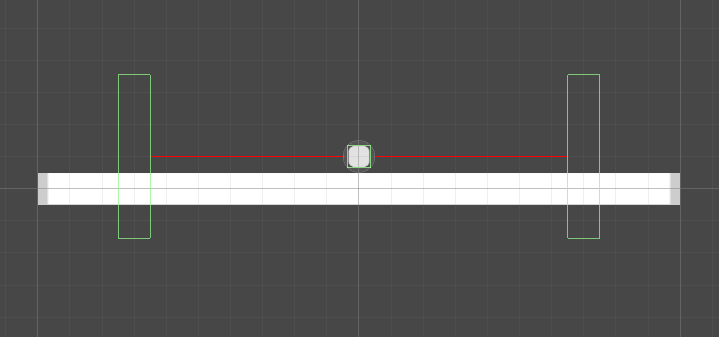
\includegraphics[width=\textwidth]{images/NPC_scene.png} 
    
    \newpage

    \subsection{ Autonomia en el moviment }
    
    \subsubsection{ Versió (I) }
    
   Els mètodes que s'hi han sobreescrit de la classe \textit{Agent} són els següents:
    
    \begin{itemize}
        \item Initialize
        \item OnEpisodiBegin
        \item OnActionReceived
        \item CollectObservations
        \item Heuristic
    \end{itemize}
    
    Altres mètodes de classe no propis de la classe \textit{Agent} i que són interessants per poder explicar la modelització del problema:
    
    \begin{itemize}
        \item OnTriggerEnter2D
        \item OnTriggerExit2D
    \end{itemize}
    
    \paragraph{Initialize}
    
   Rutina que s'executa només un cop quan es dona play al motor d'Unity.

    Agafo el component de l'objecte que em permet treballar amb les físiques de Unity. El component és el \textit{RigidBody} que ha d'haver estat afegit a l'objecte com una component des de l'interficie d'Unity. El component \textit{RigidBody} ha de tenir el comportament de \textit{Dynamic} perquè sigui afectat per la gravetat de configurada en l'escena.
    
    Per altra banda configuro el nombre de passos per episodi a zero, en cas que l'estat de la variable \textit{trainingMode} sigui fals. Aquesta configuració em permet fer proves en mode \textit{Heuristic} o en mode \textit{Inferencia} sense passar pel cicle de vida \textit{OnEpisidoBegin}.
    
    La variable \textit{MaxStep} és una variable pròpia de la classe \textit{Agent} i representa el nombre de passos màxims que es fan durant l'Agent està aprenent una política. Quan s'ha fet aquests nombres de passos, immediatament pel cicle de vida de l'Agent, força l'execució de la rutina \textit{OnEpisodiBegin}. \\
    
    \begin{lstlisting}
    public override void Initialize()
    {
        _rigidbody2D = GetComponent<Rigidbody2D>();
        // infinite steps for session
        if (!trainningMode) MaxStep = 0;
    }
    \end{lstlisting}
    
    
    \newpage
    
    \paragraph{OnEpisodeBegin}
    
    El següent mètode s'executa a l'inici de cada episodi. És important de restablir els estats inicials d'algunes propietats de l'Agent, degut a què l'Agent manté la inèrcia del episodi anterior.

    En la rutina es treu l'inèrcia que tenia l'Agent en l'episodi anterior, se'l reposiciona al centre i s'escull una meta aleatòriament. A aquestes altures les metes a escollir són els límits.
    
    \begin{lstlisting}
    public override void OnEpisodeBegin()
    {
        // reseting movement inercy
        _rigidbody2D.velocity = Vector2.zero;
        //reseting positions
        transform.position = transform.parent.position;
        // changin randomnes
        Random.InitState(System.DateTime.Now.Millisecond);
        // finding the moving target
        FindMovingTarget();
    }
    \end{lstlisting}
    
    \paragraph{OnActionReceived}
    
    La lògica dintre d'aquests mètode determina el comportament de l'Agent.
    Les accions que s'esperen és una continua, un valor entre menys u i més u. Segons aquesta acció la velocitat de l'Agent serà donada.
    
    \begin{lstlisting}
    // called when action is received from either {player, neural network}
    // each buffer position refers to an action, I decide what it means for each positions
    // inside that structure has continuous and discrete actions
    // index 0: -1 means move to the left, +1 means move to the right
    // the cool thing about the neural network, is that it figures it all automatic
    public override void OnActionReceived(ActionBuffers actions)
    {
        Vector2 movement = new Vector2(actions.ContinuousActions[0] * movementForce, 0);
        _rigidbody2D.velocity = movement;
    }
    \end{lstlisting}
    
    \paragraph{CollectObservations}
    
    En aquest mètode li he de donar al procés d'aprenentatge aquells paràmetres que jo crec que són importants per tenir en compte a l'hora d'aprendre la política.

    Aquí vaig trobar interessant d'informar el procés d'aprenentatge, quina és la horientació del Agent respecte el punt objectiu. La distància de l'Agent respecte el punt objectiu, la posició del punt objectiu i finalment la velocitat de moviment de l'Agent.
    
    \begin{lstlisting}
    // Should include all variables relevant for following 
    // to take the agent the optimally informed desition.
    // No extraneous information here please
    public override void CollectObservations(VectorSensor sensor)
    {
        if (!currentTarget) return;

        Vector2 currentPos = new Vector2(transform.position.x, 0);
        Vector2 targetPos = new Vector2(currentTarget.position.x, 0);

        Vector2 toTarget = targetPos - currentPos;
        // 2 observations (horientation)
        sensor.AddObservation(toTarget.normalized);
        // 1 observation (distance)
        sensor.AddObservation(Vector2.Distance(targetPos, currentPos));
        // 2 observations for current target position
        sensor.AddObservation(targetPos);
        // 2 observations for movement velocity
        sensor.AddObservation(_rigidbody2D.velocity);
        // Note: curiosamente si normalizo la velocidad, le cuesta mucho aprenderx
    }
    \end{lstlisting}
   
   \newpage
   
   \paragraph{Heuristic}
   En aquesta versió únicament l'Agent ha de poder interpretar valors entrats per teclat que representin moviments laterals.
    
    Es modifica la referència dels \textit{ActionBuffers} de tal manera que en el buffer de variables contínues és passa el valor entrat per teclat. \\
   
   \begin{lstlisting}
   // this method allows me to interact with the game
    // when the ml agents is not set to trainning
    public override void Heuristic(in ActionBuffers actionsOut)
    {
        ActionSegment<float> continuosActions = actionsOut.ContinuousActions;
        var force = Input.GetAxis("Horizontal");
        continuosActions[0] = force;
    }
   \end{lstlisting}
   
   \newpage
    
    \subsection{Metodologia i Resultats}
    
    \subsubsection{Autonomia en el moviment, versió (I)}
    L'objectiu de fer aprendre la política de moure's cíclicament ha sigut tot un èxit.
    
    Perquè el temps d'aprenentatge es fes més curt, el que vaig fer va ser duplicar l'Agent quatre vegades. \\
        
    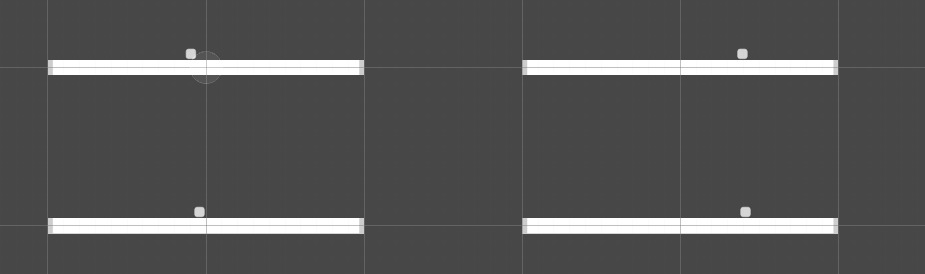
\includegraphics[width=\textwidth]{images/v1/autonomia_v1.jpeg}
    
    Fixem-nos en els següents logs que \textit{mlagents-learn} va soltant en el procés d'aprenentatge. \\
    
    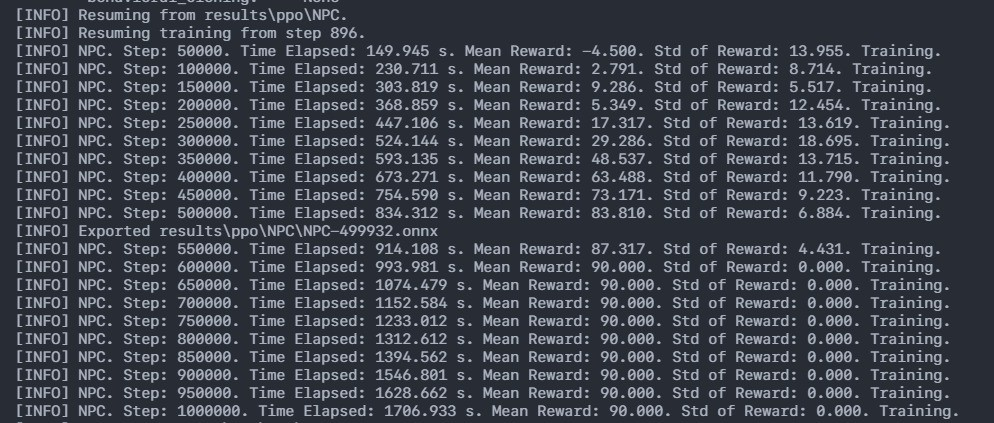
\includegraphics[width=\textwidth]{images/v1/log_v1.jpeg}
    
    Cada una de les entrades del log representen episodis. Les primeres entrades donen una mitja \textit{Mean Reward} que les últimes i la desviació estàndard és bastant més ample que les últimes.
    
    Finalment arriba el moment on l'aprenentatge de l'Agent no canvia. Això vol dir que ha après una política i immediatament, \textit{mlagents-learn} quan veu que la mitja per cada episodi és la mitja tanca el procés d'aprenentatge.
    
    \newpage
    A continuació veurem algunes gràfiques que \textit{Tensorboard} ens ha generat respecte a aquest procés d'aprenentatge.
    
    \begin{figure}[H]
        \begin{figure}[H]
        \centering
            \subcaptionbox{Comulative reward}{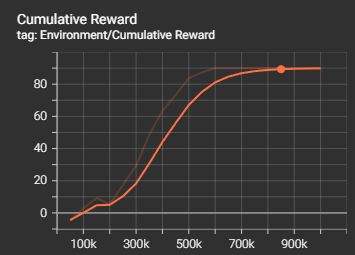
\includegraphics[width=0.30\textwidth]{images/v1/comulative_reward_autonomia_v1.png}}%
            \hfill % <-- Seperation
            \subcaptionbox{Episodi length}{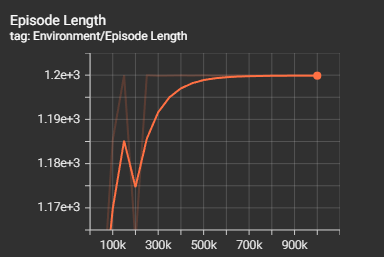
\includegraphics[width=0.30\textwidth]{images/v1/episode_length_autonomia_v1.png}}%
            \hfill % <-- Seperation
            \subcaptionbox{Learning rate}{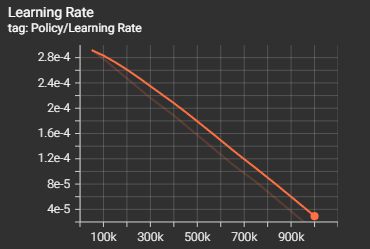
\includegraphics[width=0.30\textwidth]{images/v1/learning_rate_v1.png}}%
            \hfill % <-- Seperation
             \subcaptionbox{Policity loss}{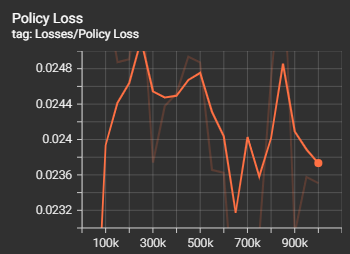
\includegraphics[width=0.30\textwidth]{images/v1/policity_loss_autonomia_v1.png}}%
            \hfill % <-- Seperation
            \subcaptionbox{Value Loss}{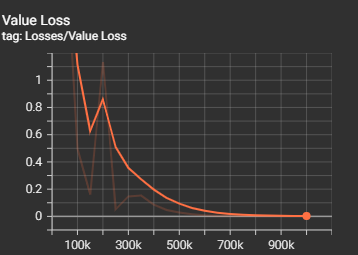
\includegraphics[width=0.30\textwidth]{images/v1/value_loss_autonomia_v1.png}}%
            \hfill % <-- Seperation
            \subcaptionbox{Entropy}{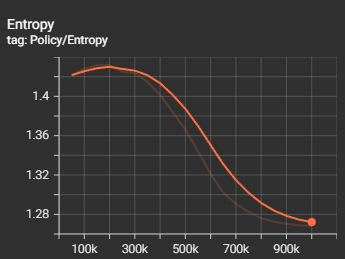
\includegraphics[width=0.30\textwidth]{images/v1/entropy_autonomia_v1.png}}%
            
        \end{figure}
    \end{figure}

          
    \section{Conclusions i línies futures}
    
    \section{Referències}

\end{document}
